
\PassOptionsToPackage{dvipsnames}{xcolor}
\documentclass[aspectratio=169,11pt]{beamer}
\newcommand{\teamname}{VerteX}
\newcommand{\topicchoice}{Async Research Assistant}
\newcommand{\reportdate}{16 September 2026}
\newcommand{\repolink}{github.com/yagubbx/Research-Assistant}
\newcommand{\memberone}{Yaqub Xəlilli}
\newcommand{\membertwo}{Səbuhi Xamiyev}
\newcommand{\memberthree}{Aqil Əsgərov}








\newcommand{\coursecode}{AI-ENG-110}
\newcommand{\coursename}{Software Engineering}
\newcommand{\institution}{AI Academy, National AI Center}
\newcommand{\semester}{Spring 2026}

\usepackage{fontspec}
\setmainfont{NotoSerif}[Path=../docs/fonts/,Extension=.ttf,UprightFont=*-Regular,BoldFont=*-Bold,ItalicFont=*-Italic,BoldItalicFont=*-BoldItalic]
\setsansfont{NotoSans}[Path=../docs/fonts/,Extension=.ttf,UprightFont=*-Regular,BoldFont=*-Bold,ItalicFont=*-Italic,BoldItalicFont=*-BoldItalic]
\setmonofont{texgyrecursor-regular.otf}

\usepackage{xcolor}
\usepackage{tabularx}
\usepackage{booktabs}
\usepackage{listings}
\usepackage{tikz}
\usetikzlibrary{shapes.geometric,arrows.meta,positioning,fit,backgrounds}

\definecolor{accent2}{HTML}{8B0000}


\usetheme{default}
\usefonttheme{professionalfonts}
\setbeamertemplate{navigation symbols}{}

\definecolor{accent}{HTML}{0B3D91}
\definecolor{soft}{HTML}{F2F4F8}
\definecolor{ok}{HTML}{166534}

\setbeamercolor{title}{fg=accent}
\setbeamercolor{frametitle}{fg=accent}
\setbeamercolor{section in head/foot}{bg=accent,fg=white}
\setbeamercolor{itemize item}{fg=accent}
\setbeamercolor{itemize subitem}{fg=accent}
\setbeamercolor{enumerate item}{fg=accent}
\setbeamercolor{block title}{bg=accent,fg=white}
\setbeamercolor{block body}{bg=soft,fg=black}

\setbeamerfont{title}{size=\Large,series=\bfseries}
\setbeamerfont{frametitle}{size=\large,series=\bfseries}
\setbeamerfont{footline}{size=\tiny}

\setbeamertemplate{footline}{%
  \leavevmode%
  \hbox to \paperwidth{\hspace*{2ex}\tiny\textit{\teamname{} -- \topicchoice}\hfill%
  \tiny\textit{\coursecode{} -- \semester{}}\hfill%
  \tiny\insertframenumber/\inserttotalframenumber\hspace*{2ex}}%
  \vskip1pt%
}

\definecolor{codegreen}{rgb}{0,0.55,0}
\definecolor{codepurple}{rgb}{0.55,0,0.78}
\lstdefinestyle{python}{
  language=Python,
  backgroundcolor=\color{soft},
  commentstyle=\color{codegreen},
  keywordstyle=\color{accent},
  stringstyle=\color{codepurple},
  basicstyle=\ttfamily\scriptsize,
  breaklines=true,
  frame=single,
  framerule=0.4pt,
  rulecolor=\color{black!30},
}

\usepackage{xurl}
\begin{document}

{\setbeamertemplate{footline}{}
\begin{frame}[plain]\centering
{\small AI Academy, National AI Center\\AI-ENG-110 -- Software Engineering}\\[0.8cm]
\rule{0.75\textwidth}{0.6pt}\\[0.4cm]
{\Huge\bfseries\color{accent}Async Research Assistant}\\[0.4cm]
\rule{0.75\textwidth}{0.6pt}\\[0.6cm]
{\Large VerteX}\\[0.4cm]
Yaqub Xəlilli \quad Səbuhi Xamiyev \quad Aqil Əsgərov\\[0.6cm]
{\small github.com/yagubbx/Research-Assistant}
\end{frame}}

\begin{frame}{Research Assistant: purpose and workflow}
\textbf{One question, evidence from several sources.}\\[0.12cm]
A concise answer with numbered references the user can inspect.
\vspace{0.38cm}
\begin{columns}[T,onlytextwidth]
\column{.29\textwidth}
{\color{accent}\textbf{01\quad Ask}}\\[0.18cm]
Enter a research question.\\[0.18cm]
Choose Wikipedia, arXiv or web sources.\\[0.18cm]
Use the CLI or Streamlit UI.
\column{.32\textwidth}
{\color{accent}\textbf{02\quad Research}}\\[0.18cm]
Fetch selected sources concurrently.\\[0.18cm]
Reuse valid cached evidence.\\[0.18cm]
Generate an answer with an LLM.
\column{.31\textwidth}
{\color{accent}\textbf{03\quad Inspect}}\\[0.18cm]
Read the answer and open its references.\\[0.18cm]
See source status and timing.\\[0.18cm]
Export text or JSON.
\end{columns}
\vspace{0.38cm}
{\small\color{accent}\textbf{When a source fails:} usable evidence remains available, with a visible note.}
\vspace{0.18cm}

{\footnotesize Live research needs internet and an API key. Offline mode uses five labeled sample topics.}
\end{frame}

\begin{frame}{Architecture}
\centering\resizebox{.92\textwidth}{!}{\begin{minipage}{15cm}
\begin{center}
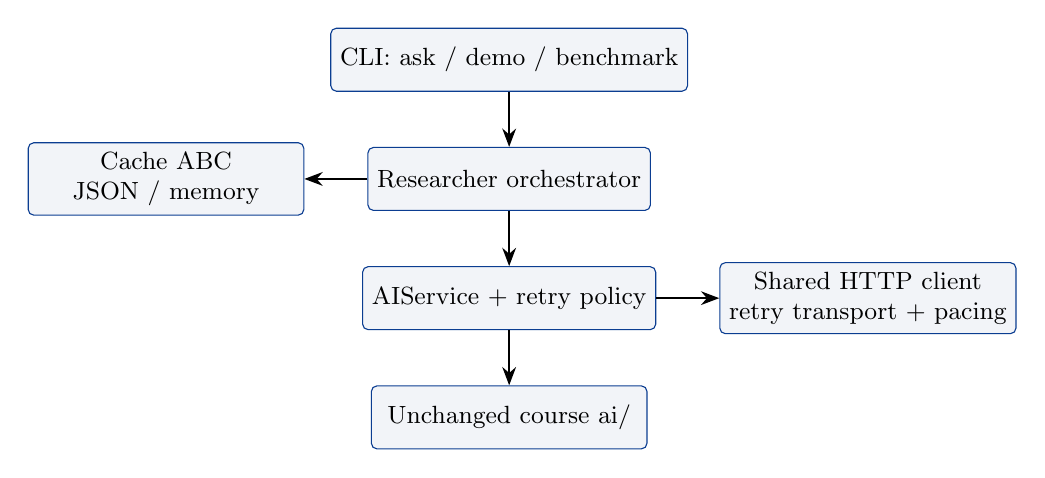
\begin{tikzpicture}[node distance=7mm,box/.style={draw=accent,rounded corners=2pt,fill=soft,align=center,minimum width=3.5cm,minimum height=8mm,font=\small},arr/.style={-Stealth,thick}]
\node[box] (cli) {CLI: ask / demo / benchmark};
\node[box,below=of cli] (core) {Researcher orchestrator};
\node[box,left=8mm of core] (cache) {Cache ABC\\JSON / memory};
\node[box,below=of core] (service) {AIService + retry policy};
\node[box,below=of service] (ai) {Unchanged course ai/};
\node[box,right=8mm of service] (http) {Shared HTTP client\\retry transport + pacing};
\draw[arr] (cli)--(core); \draw[arr] (core)--(cache);
\draw[arr] (core)--(service); \draw[arr] (service)--(ai); \draw[arr] (service)--(http);
\end{tikzpicture}
\end{center}
\end{minipage}}
\vspace{0.3cm}
\small Pydantic models cross boundaries. Only the service and its worker call the supplied AI package. No changes to \texttt{ai/}.
\end{frame}

\begin{frame}{Design decisions}
\begin{enumerate}\setlength\itemsep{0.65cm}
\item \textbf{Async I/O for retrieval}\\Independent sources overlap; a semaphore caps active operations.
\item \textbf{Filesystem cache behind an interface}\\Persistence without a database server; memory backend supports tests.
\item \textbf{A process for synchronous synthesis}\\A deadline can terminate the SDK call; startup adds latency.
\end{enumerate}
\end{frame}

\begin{frame}{Retrieval benchmark}
\textbf{Five questions, three repetitions, cache bypassed}\vspace{0.4cm}
\begin{center}\begin{tabular}{lrr}\toprule & Sequential & Parallel\\\midrule
Median seconds & 2.412 & 0.802\\Speedup & 1.00$\times$ & 3.01$\times$\\Failed / empty & 0 & 0\\\bottomrule\end{tabular}\end{center}
\vspace{0.35cm}
Synthetic HTTP delays: 150 ms per source; semaphore = 3.\\
\textbf{Scope:} retrieval only; no live-provider latency claim.\\[0.3cm]
\textbf{Bottleneck:} the slowest source after overlap; synthesis may dominate the full live run.
\end{frame}

\begin{frame}{Integration problems and solutions}
\begin{itemize}\setlength\itemsep{0.35cm}
\item \textbf{Uncited sentences:} validate and regenerate within the existing retry budget; never invent citations.
\item \textbf{Empty or slow search:} simplify topic queries; bound web search in a killable worker.
\item \textbf{Gemini errors:} inspect safe status codes; align model defaults with the working deployment.
\item \textbf{Source failure:} keep usable evidence and show a missing-source note; stop if all sources fail.
\end{itemize}
\small Evidence: regression tests, Docker acceptance log and Render live sample.
\end{frame}

\begin{frame}[fragile]{Scripted demonstration}
\begin{lstlisting}[style=python,language=bash,numbers=none]
python -m streamlit run researcher/web_ui.py
python -m researcher ask "photosynthesis" \
  --offline --sources wiki,arxiv --json
docker run --rm --network none vertex-research
\end{lstlisting}
\vspace{0.4cm}
Five original questions produce answers with numbered references.\\[0.25cm]
Offline evidence is visibly labeled \textbf{SIMULATED}.\\[0.25cm]
\small Render live sample: 23.21 s, 3 sources, 3 references. Offline mode needs no key.
\end{frame}

\begin{frame}{Testing evidence}
\begin{columns}[T,onlytextwidth]
\column{.46\textwidth}{\Huge\color{accent}121} passing tests\\[0.45cm]
{\Huge\color{accent}93.85\%} application coverage\\[0.35cm]
16 unchanged course smoke tests included.
\column{.48\textwidth}\textbf{High-value checks}\begin{itemize}\item Source failure and timeout\item Semaphore bound and overlap\item 429 recovery; no 401 retry\item Cache expiry and corruption\item Invalid and missing citations\end{itemize}
\end{columns}\vspace{0.5cm}
\small Ruff passes; mypy reports no issues in 18 files. Tests use mocks and deny live sockets.
\end{frame}

\begin{frame}{Tested extensions in v1.1.0}
\begin{itemize}\setlength\itemsep{0.3cm}
\item \textbf{Web failover:} primary failure or timeout, then a configured secondary; chaos tests verify recovery.
\item \textbf{Token budget:} estimated sliding-window reservations; exhaustion test observes 60 s backoff.
\item \textbf{Streamlit:} same core pipeline, sample/live modes, references and downloads; AppTest and browser checks.
\item \textbf{CI:} lint, types, tests, coverage and container UI health workflow.
\end{itemize}\vspace{0.2cm}
\small Docker acceptance passed. Live Gemini passed; PR 1 checks passed before merge. Bonus credit is assessed by the instructor.
\end{frame}

\begin{frame}{Team and AI disclosure}
\begin{tabularx}{\textwidth}{lX}\toprule
Member & Responsibility (team-reported)\\\midrule
Yaqub Xəlilli & CLI/core, integration and deploy\\
Səbuhi Xamiyev & Providers, worker, retry and search\\
Aqil Əsgərov & Cache, validation, offline and UI\\\bottomrule\end{tabularx}\par
\vspace{0.5cm}
Codex substantially drafted the software, tests and documentation.\\[0.3cm]
Team reports about 90\% joint sessions; implementation commits centralized under Yaqub. The signed contribution statement is included in the final release.\\[0.4cm]
\textbf{Defense goal:} every member can explain the full request path.
\end{frame}

{\setbeamertemplate{footline}{}
\begin{frame}[plain]
\begin{columns}[c,onlytextwidth]
\column{.51\textwidth}
{\Huge\bfseries\color{accent}Live demonstration}\\[0.45cm]
{\Large Async Research Assistant}\\[0.35cm]
Scan the QR code to open\\the deployed application.\\[0.45cm]
{\large\bfseries VerteX}\\[0.25cm]
{\small Questions and discussion}
\column{.43\textwidth}
\centering
\href{https://vertex-research-assistant.onrender.com/}{
\includegraphics[width=4.9cm]{render-qr.png}}\\[0.12cm]
{\small\color{accent}\href{https://vertex-research-assistant.onrender.com/}{Open the live application}}
\end{columns}
\vspace{0.45cm}
\centering
{\small\href{https://vertex-research-assistant.onrender.com/}{vertex-research-assistant.onrender.com}}\\[0.15cm]
{\small Repository: \href{https://github.com/yagubbx/Research-Assistant}{github.com/yagubbx/Research-Assistant}}
\end{frame}}
\end{document}